\documentclass{article}
\usepackage{amsmath}
\usepackage{listings}
\usepackage{amssymb}
\usepackage{color}
\usepackage{graphicx}
\parindent=19pt
\begin{document}
\title{Finite Element Method}
\author{Wei Zhang}
\large
\maketitle


\section{Exercise 17: Compute the deflection of a cable with sine functions}
The problem is
\begin{gather}
u''=1, x\in(0, 1), \qquad  u(0)=0, \quad u'(1)=0
\end{gather}
We choose the base functions $\varphi_{i}=\sin((i+1)\pi x/2)$, $i=1, \ldots, N.$\\
\subsection{Galerkin method:}
\begin{center}
$u\approx \hat{u}=0+\displaystyle \sum^{N}_{j=1}u_{j}N_{j}(x)$
\end{center}
with $N_{j}(0)=0$. We choose weighting function $W_{i}=N_{i}$. This leads to:
\begin{gather}
\displaystyle \sum^{N}_{j=1}\left(\int^{1}_{0} N_{i}N''_{j}(x)dx\right)u_{j}=\int^{1}_{0} N_{i}dx, \qquad i=1, \ldots, N.
\end{gather}
Integrating by parts on the left side
\begin{gather}
\displaystyle -\sum^{N}_{j=1}\left(\int^{1}_{0} N'_{i}N'_{j}(x)dx\right)u_{j}+N_{i}(1)\hat{u}'(1)-N_{i}(0)\hat{u}'(0)=\int^{1}_{0} N_{i}dx, \quad i=1, \ldots, N.
\end{gather}\\
Since $\hat{u}'(1)=0$, $N_{i}(0)=0$, we get
\begin{gather}
\displaystyle \sum^{N}_{j=1}\left(\int^{1}_{0} N'_{i}N'_{j}(x)dx\right)u_{j}=-\int^{1}_{0} N_{i}dx, \quad i=1, \ldots, N.
\end{gather}
We get a linear system $\textbf{A}u=\textbf{b}$, with
\begin{gather}
 A_{i,j}=\displaystyle\int^{1}_{0}N'_{i}N'_{j}(x)dx, \qquad
\displaystyle b_{i}=-\int^{1}_{0} N_{i}dx.
\end{gather}
\subsection{Least Squares Method:}
The residual
\begin{equation}
R=\displaystyle \sum^{N}_{j=1}u_{j}N''_{j}(x)-1
\end{equation}
the derivative
\begin{equation}
\displaystyle \frac{\partial R}{\partial u_{i}}= \sum^{N}_{j=1}\frac{\partial}{\partial u_{j}}N''_{j}(x)=N''_{i}(x)
\end{equation}
the least squares equation
\begin{equation*}
\displaystyle  \int^{1}_{0}\left(\sum^{N}_{j=1}u_{j}N''_{j}(x)-1\right)N''_{i}(x)dx=0
\end{equation*}

\begin{gather}
\displaystyle  \sum^{N}_{j=1} \left(\int^{1}_{0}N''_{i}(x)N''_{j}(x)dx\right)u_{j}=\int^{1}_{0}N''_{i}dx, \qquad i=1, \ldots, N.
\end{gather}
We get a linear system $\textbf{A}u=b$, with
\begin{gather}
A_{i,j}=\displaystyle\int^{1}_{0}N''_{i}N''_{j}(x)dx, \qquad
\displaystyle b_{i}=\int^{1}_{0}N''_{i}dx.
\end{gather}
The results when using one basis function are shown in Figure 1.
\begin{figure}[H]
\begin{center}
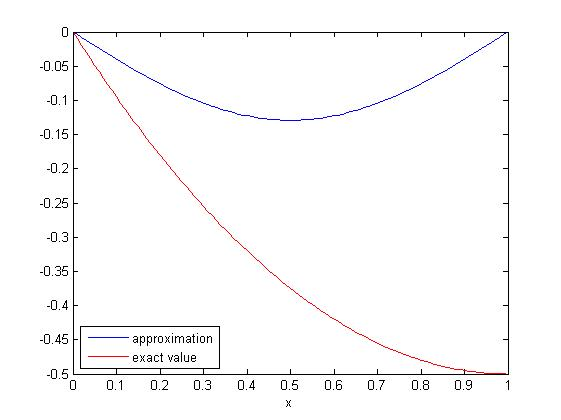
\includegraphics[width=10cm]{ex17.jpg}    % The printed column width is 8.4 cm.
\caption{Compute the deflection of a cable with using one basis function}
\end{center}
\end{figure}
\par
If we choose basis functions $\varphi_{i}=\sin((i+1)\pi x)$, the matrix \textbf{A} will become diagonal matrix since the basis functions are orthogonal
\begin{gather}
\varphi_{i}\varphi_{j}=0,  \qquad i\neq j
\end{gather}
\end{document}

